	\section{RC Week 2}
		\subsection{OK, VE280. What is this course?}
		\begin{frame}
	\frametitle{How to write good code ${}^\text{and linked lists}$}	
	\begin{block}{Writing Quality Code}
		\begin{description}[Motivation]
					\item[Taste] What kind of code are considered "good"?
					\item[Motivation] What benefit would such code give us?
					\item[Techique] What is the recipe for such code?
					\item[Tools] What language features does C++ provide for achieving this goal? How to use them?
				\end{description}
				\small{Good (Bad?) News: Exams will (mostly) test for the last point.}
			\end{block}
			\begin{block}{Elementary Data Structure}
				Singly linked lists, Doubly linked lists, Circular Arrays ... \
			\end{block}
		\end{frame}
		\begin{frame}{OK, "Quality Code"?}
			It's very hard to give a definition.
			\begin{columns}
				\column[]{.5\textwidth}
				
				\begin{block}{Good Code}
					\begin{itemize}
						\item Good variable names
						\item Consistent indentation
						\item Well tested, documented
						\item D-R-Y, Don't repeat yourself
						\item High Coherence / Low coupling
						\item Open for extension, but closed for modification
					\end{itemize}
				\end{block}
				\column[]{.5\textwidth}
				\begin{block}{Bad Code}
					\begin{itemize}
						\item Bad Style
						\item 200+ lines in a one function
						\item Functions of 20+ Args
						\item Magic numbers everywhere
						\item Seriously you know bad code when you see one (write one).
					\end{itemize}
				\end{block}
			\end{columns}
			Many of them are related to \emph{Abstraction}.
		\end{frame}
	
\begin{frame}[fragile]{Head First \textit{Abstraction}}
	\framesubtitle{No abstraction}
	\begin{block}{The Requirement}
		\textit{CubedEnix (CE)} is trying to develop a third person shooting game called \textit{World of Armored Blizzard} (WOAB). In this game, AI will control a tank that can fire upon the player. A programmer \textit{Archer} is asked to implement this feature. 
	\end{block}
	\begin{block}{The Solution}
		Archer propose to have a global variable \texttt{TANK} of class \texttt{Tank} to represent the tank. Archer than writes the following code.
\begin{minted}{c++}
...
Player target = TANK.aim(); TANK.fire(target);
...
\end{minted}
		Archer feels happy, so does his boss.
	\end{block}
\end{frame}

\begin{frame}[fragile]{Head First \textit{Abstraction}}
	\framesubtitle{No abstraction}
	\begin{block}{Change of Requirement}
		Players are complaining that the game is too easy. WOAB dev team decided to add 2 more AI controlled tanks. Again Archer is asked to implement it.
	\end{block}
	\begin{block}{The Solution}
		Archer decided to use 3 global variables \texttt{TANK0, TANK1, TANK2} of class \texttt{Tank}. He copies the original code into 3 different places and modify each of them.
		\begin{minted}{c++}
... Player target = TANK0.aim(); TANK0.fire(target);
... Player target = TANK1.aim(); TANK1.fire(target);
... Player target = TANK2.aim(); TANK2.fire(target);
		\end{minted}
		Archer feels happy, so does his boss.
	\end{block}
\end{frame}

\begin{frame}[fragile]{Head First \textit{Abstraction}}
	\framesubtitle{No abstraction}
	\begin{block}{Change of Requirement}
		Within the next 2 months they increased number of tanks to 10. 1 year later, they (finally!) decided to play a sound effect when a tank fires. 
	\end{block}
	\begin{block}{The Twist}
		Archer now has 10 copies! He needs to add a function call \texttt{playSound()} to each copy. Unfortunately he missed one location.  Archer also doesn't test his code.  Now Buggy code is released.
		
		Players are unhappy. His boss is unhappy. Archer is fired. Archer is unhappy. Lancer takes his job.
	\end{block}
\end{frame}

\begin{frame}[fragile]{Head First \textit{Abstraction}}
	\framesubtitle{With Procedual Abstraction}
	\begin{block}{The Solution}
		Lancer decided to write a function that takes a \texttt{Tank} object as an argument.
		\begin{minted}{c++}
// Argument: A non-null pointer to a Tank object.
// Effect  : Fires such tank on the current player.
void tankFire(Tank* t) {
    playSound();
    Player target = t->takeAim(); 
    t->fire(target);
}
		\end{minted}
		With this new design Lancer can easily change the number of \texttt{TANK}s in the game, or modify the how tanks fire by simply changing this single function.
	\end{block}
\end{frame}

\begin{frame}[fragile]{Head First \textit{Abstraction}}
\framesubtitle{With just procedual abstraction}
\begin{block}{Change of Requirement}
	\small{You know what? Those player just can't be satisfied. WOAB dev team now decides to involve not just tanks but also battle ships and planes (and witches and dragons ...). Lancer is asked to implement "fire" feature for all of them.}
\end{block}
\begin{block}{The Twist}
	\small{Lancer is now in a tough situation. Clearly Tanks, Ships, Planes... are different things. Their attack would have different effects. There won't be a single function that works for all of them.
	
	Since Lancer didn't take VE280 seriously when he is in JI, Lancer falls back to copying the code for each "character" once. After 2 months, the code is no longer maintainable, and thus he is fired. Saber takes his job.}
\end{block}
\end{frame}

\begin{frame}[fragile]{Head First \textit{Abstraction}}
\framesubtitle{With Data Abstraction}
\begin{block}{The Solution}
The key is to see the elephant in the room. What's the common characteristic of tanks, ships, dragons and witches? They all attack our player!
\begin{minted}{c++}
class IAttackPlayer {
    virtual void fire(Player p) = 0;
    virtual Player takeAim() = 0;
}
class Tank : public IAttackPlayer;
class Ship : public IAttackPlayer;
....
\end{minted}
\end{block}
\end{frame}

\begin{frame}[fragile]{Head First \textit{Abstraction}}
\framesubtitle{With Data Abstraction}
\begin{block}{The Solution}
	Then we can modify the function:
	\begin{minted}{c++}
// Argument: a object implements IAttackPlayer.
// Effect  : Fires such tank on the current player.
void NpcFire(IAttackPlayer* t) {
    playSound();
    Player target = t->takeAim(); 
    t->fire(target);
}
	\end{minted}
	In the above design Saber abstracted out what the thing "physically" is. She defines things by defining what it can do.
\end{block}
\end{frame}

\begin{frame}{A few more words}
\begin{block}{It's okay if You don't fully understand above story}
	That's gives you a good reason to learn it well.
\end{block}
\begin{block}{Can you talk something about projects?}
	Well, projects are mostly very direct. Be careful in the process and they should be pretty easy. Reserve around 5 days for them. You only have a limited number of trials each day. 
	
	Remember it's easy to simply finish them. But to finish them elegantly trust me when I say it's hard. 
	
	Yes, it's hard. But the outcome worth every minute spent.
\end{block}
\end{frame}

\subsection{Your Linux Operating System}
\begin{frame}{Linux as a operating system \textit{kernel}}
\begin{block}{Operating systems as a resource manager}
	Operating systems manages your hardware. These includes computation resource (CPU, GPU), storage (Hard drive), communication resource (network)...
\end{block}
\begin{block}{The core of OS, a.k.a. \textit{kernel}}
	At the very heart of the OS there lies the kernel. This piece of software talks directly to the hardware. It provides a unified way of accessing your storage devices (Filesystems), graphic devices, network...
\end{block}
\begin{block}{``Linux" is first the name of the kernel}
	This implies you can actually change your desktop environment: fancier? go with Unity/KDE/Gnome. Light weight \& fast? go with LXDE or XFCE. 
\end{block}
\end{frame}

\begin{frame}{Flavors of Linux: \textit{Distributions}}
\framesubtitle{Common Choices}
\begin{small}
	This flexibility of choice allows to tailor the system towards our own need. Some commonly accepted configurations become "Distributions".
\end{small} 
\begin{block}{Ubuntu Series}
	Maintained by Canonical, it's actually a series of distributions with different choice of desktop environment. Ubuntu / \textit{Unity}. Kubuntu / \textit{KDE}. Lubuntu / \textit{LXDE}. Xubuntu / \textit{XFCE}. Use \textit{apt}.
\end{block}
\begin{block}{Debian}
	Once the most widely use distribution, the father of Ubuntu [that's right :=)]. Package management system is \textit{apt}
\end{block}
\begin{block}{Fedora and RedHat Linux Enterprise}
	Maintained by Red Hat. Fedora is new and cutting edge. RedHat now focus on enterprises. Package Management is \textit{yum}.
\end{block}
\end{frame}

\begin{frame}{Flavors of Linux: \textit{Distributions}}
\framesubtitle{Uncommon choices}
\begin{block}{Open SUSE}
	Maintained by german company SUSE. Focus on stability. 
\end{block}
\begin{block}{Arch Linux}
	ROLLING UPDATE! Absolutely cutting edge. Great community and wiki. User is assumed to be experienced. Installation is done on command line. Package management system is \textit{pacman}.
\end{block}
\begin{block}{Linux From Scratch}
	Try this if you are absolutely interested in figuring out how everything works.
\end{block}
\begin{block}{Gentoo}
	Think LFS is crazy enough? Well this things compiles every piece of software you use FROM THE SOURCE! 
\end{block}
\end{frame}

\begin{frame}{Bash on Windows Subsystem for Linux}
\begin{block}{Think big, with abstraction}
	For Linux programs, technically, you don't need an "real" linux kernel to run them. As long as you have some thing that looks like a real one (one that follows the same abstraction). 
\end{block}
\begin{block}{Windows Subsystem for Linux}
	This year Microsoft actually release one. Installation guide is available \href{https://msdn.microsoft.com/zh-cn/commandline/wsl/install\_guide}{here(click me)}.
	
	This solution is easy to use, clean. It saves you time copying files back and forth from the virtual machine. You can simply develop in Windows using your favorite tool (IDE and test it easily under ``Linux''. It's a good solution for the purpose of this course.
\end{block}
\end{frame}

\begin{frame}[fragile]{Aspects of Linux: Users}
\vspace{-0.12in}
\begin{description}[Permission]
	\small
	\item[MultiUser] Multiple person can operate the system at once.
	\item[Group] Each User belongs to one or more groups
	\item[Home Dir] Each user has his/her own directory under \texttt{/home}
	\item[$\sim$/] Shorthand for home directory. This one is user specific.
	\item[Premission] Owner/Group/Other Read/Write/Execute Flags
	\item[root] A special super user \texttt{root} overrides all security 
	\item[su] Command that starts a temporary shell as \texttt{root}
	\item[sudo] A command that temporarily grant superuser privilege to current user. Namely, ``execute the following command as `root`". 
\end{description}
\small{The Miranda warning of \texttt{sudo}:}
\begin{minted}[fontsize=\footnotesize]{text}
We trust you have received the usual lecture from the local 
System Administrator. It usually boils down to these three things:
	#1) Respect the privacy of others.
	#2) Think before you type.
	#3) With great power comes great responsibility.
root's password:
\end{minted}
\end{frame}

\begin{frame}{Aspects of Linux: Filesystem}
\begin{block}{Filesystem is an abstraction of storage}
	That's right, abstraction again. Filesystem hides the physical storage schema of your files. Instead it should reflect how your files are logically organized.
\end{block}
\begin{block}{Linux Filesystem}
	In Linux files are organized in a tree-like structure.
	\begin{figure}
		\vspace{-0.2in}
		\centering
		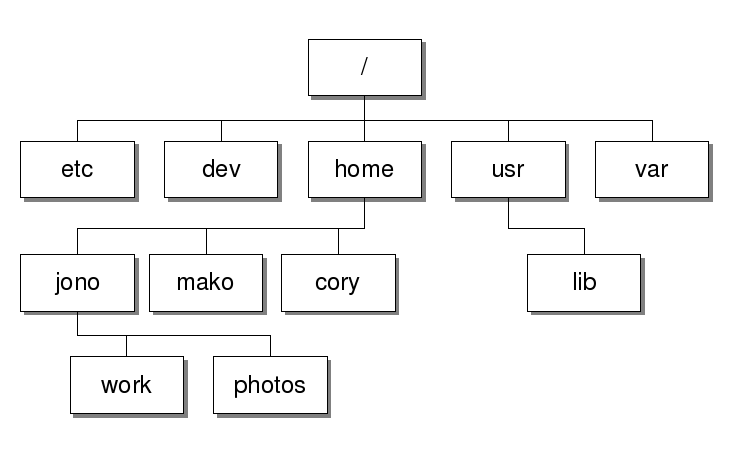
\includegraphics[scale=0.5]{fig/rc2_linuxfs}
	\end{figure}
\end{block}
\end{frame}

\begin{frame}{Aspects of Linux: Filesystem}
\framesubtitle{Caveats for the names}

\begin{block}{A word from Ken Thompson}
\begin{quote}
	Ken Thompson was once asked what he would do differently if he were redesigning the UNIX system. His reply: "I'd spell creat with an e."
\end{quote}
\end{block}

\vspace{-0.15in}
\begin{columns}
	\column{.5\textwidth}
	\begin{description}[/boot]
	\item[/bin] \textbf{Bin}aries
	\item[/dev] \textbf{Dev}ices
	\item[/lib] \textbf{Lib}raries
	\item[/boot] \textbf{Boot}strap
	\item[/sbin] \textbf{S}ecure \textbf{bin}aries
	\end{description}
	\column{.5\textwidth}
	\begin{description}[/home]
	\item[/mnt] \textbf{M}ou\textbf{nt}ed filesystem
	\item[/etc] Configuration files
	\item[/lib] \textbf{Lib}raries
	\item<2->[/usr] \textbf{U}nix \textbf{s}ystem \textbf{r}esources
	\item<2->[/home] Places for the user's files
	\end{description}
\end{columns}

\vspace{0.1in} \tiny{More at https://wiki.debian.org/FilesystemHierarchyStandar}
\end{frame}

\begin{frame}{Aspects of Linux: Shell}

\begin{block}{CLI and Shell}
\textbf{C}ommand \textbf{L}ine \textbf{I}nterface is fast, consumes minimum resources and effective. \textbf{G}raphical \textbf{U}ser \textbf{I}nterface comes with a much larger cost. 

Management tasks are generally easier on CLI (think about coding!).

The program that interprets user commands and provides feedbacks is called a \textit{Shell}. When you login to the computer, the shell runs automatically. You interact with the computer through the shell. 
\end{block}

\begin{block}{Differenct choices of shell}
	The ``standard" one on most linux is \texttt{bash}, as in ``\textbf{B}ourn's \textbf{A}nother \textbf{Sh}ell". But choices like \texttt{zsh}, \texttt{fish}, \texttt{csh} are much more easier to use (cooler). Checkout the ``oh-my-zsh" project on GitHub if you are interested.
\end{block}
\end{frame}

\begin{frame}{Aspects of Linux: Shell}
\framesubtitle{The working directory}
	How does \texttt{fopen("test.txt")} work? I mean, how does the computer know where to find \texttt{text.txt}? 
	
	Each program is associated with a special directory called ``working directory". Normally this is the directory where you execute the program. (Not where the program is!). 

\begin{block}{Related commands}
	\small
	\begin{description}[pwd]
		\item[pwd] \textbf{P}rint \textbf{w}orking \textbf{d}irectory
		\item[cd] \textbf{C}hange \textbf{d}irectory. Each directory has 2 very special ``sub-directory". ``\textbf{./}" and ``\textbf{../}". They are logically sub-directory. Meaning you can do \texttt{cd /home/john/./} and \texttt{cd /home/john/../}, but the in fact, the first command takes you to \texttt{/home/john/} and the second one takes you to \texttt{/home/}. 
		
		``\texttt{cd ./}" keeps where you are and ``\texttt{cd ../}"" takes you 1 level up.
	\end{description}
	

\end{block}
\end{frame}

\begin{frame}[fragile]{Aspects of Linux: Shell}
\framesubtitle{Executing programs}
The general syntax is 
\begin{minted}{bash}
executable_file arg1 arg2 arg3 ...
\end{minted}
Conventions are:\\
1) arguments begin with \texttt{-} are called "switches" or "options" \\
2) one dash (one \texttt{-}) are called short switches, e.g. \texttt{-l}, \texttt{-a}\\
3) short switch always uses single letter to specify. Case / lower letters can have very different meanings! Be very careful.
3) multiple short switches can often be specified at once. e.g. \texttt{ls -al}\\
4) two dashes (one \texttt{-}) are called long switches, e.g. \texttt{--all}, \texttt{--mode=linear}. Usually long switches use whole words other than acronyms.\\
5) \textbf{THERE ARE OUTLIERS!}. Unfortunately \texttt{gcc} and \texttt{g++} are two of these naughty boys. 
\end{frame}

\begin{frame}{Aspects of Linux: Shell}
\framesubtitle{Useful commands}
	\begin{description}[mkdir]
		\item[ls] \textbf{L}i\textbf{s}t files \& folders under a directory. This command takes zero or more arguments. If the argument is a directory, list that dir. If the argument is a file, show information of that specific file. If no arguments are given, list working directory.
		\begin{description}[-a]
			\small
			\item[-a] List hidden files as well. Leading dot means ``hidden".
			\item[-l] Use \textbf{l}ong format. Each line for a single file. 
		\end{description}
		\item[mkdir] \textbf{M}a\textbf{k}e \textbf{dir}ectory, self-explanatory.
		\item[rm] \textbf{R}e\textbf{m}ove files / directory. It is \textbf{extremely dangerous} to run \texttt{rm} with administrative privilege! See the bumblebee accident. \small{https://github.com/MrMEEE/bumblebee-Old-and-abbandoned/issues/123}
		\begin{description}[-a]
			\small
			\item[-r] Deletes files/folders recursively. Folders requires this option.
			\item[-f] Force remove. Ignores warnings.  
		\end{description}
		\item[rmdir] \textbf{R}e\textbf{m}ove \textbf{dir}ectory, only \textbf{empty} ones can be removed this way.
	\end{description}

\end{frame}

\begin{frame}{Aspects of Linux: Shell}
\framesubtitle{Useful commands, Cont'd}
\begin{description}[mkdir]
	\item[touch] Designed to change the time stamp of file. Commonly used to create an empty file.
	\item[cp] \textbf{C}o\textbf{p}y files/folder. Takes 2 arguments \texttt{source} and \texttt{dest}. Be very careful if both \texttt{source} and \texttt{dest} are both existing folders. Try it yourself!
	\begin{description}[-]
		\small
		\item[-r] Copy files/folders recursively. Folders requires this option.  
	\end{description}
	\item[mv] \textbf{M}o\textbf{v}e files / directory. Takes 2 arguments \texttt{source} and \texttt{dest}. If \texttt{source} and \texttt{dest} is the same location, this command essentially does a rename. Pay attention to the situation where both arguments are already existed.
	\item[cat]<2-> Con\textbf{cat}enate files. Takes multiple arguments and print their content one by one to \texttt{stdout}. When there is just one argument, it essentially displays the content.
\end{description}
\end{frame}

\begin{frame}{Aspects of Linux: Shell}
\framesubtitle{CLI Utilities}
\begin{description}[vi/vim]
	\item[nano] Command line file editor.
	\item[diff] Compare the \textbf{diff}erence of two files. 
	\begin{description}[-]
		\small
		\item[-y] A side by side view, try it yourself.
		\item[-w] Ignore white spaces.  
	\end{description}
	\item[less] Prints the content from its \texttt{stdin} in a readable way.
	\item[vi] Advanced text editor
	\item[vim] \textbf{v}i \textbf{im}proved, both \texttt{vi} and \texttt{vim} can be exited by first press \texttt{ESC} and type ``\texttt{:q!}". You should know this in case your ``friend" opens a \texttt{vi} window when you are away, so you won't get stuck inside.
	\item[grep] Filters input and extracts lines that contains specific content. Very useful in debugging programs. 
	\item[echo] Prints its arguments to \texttt{stdout}.
\end{description}

\end{frame}

\begin{frame}{Aspects of Linux: Shell}
\framesubtitle{IO Redirection}
When you are reading \texttt{cin} or writing to \texttt{cout}, you are essentially read/writing 2 special files. Again, abstraction, right? 

It is possible to ``switch" these two ``virtual files" with real files before the actual execution of the program. This is called IO ``redirection".

There are 4 most common redirections:

\begin{description}[\texttt{exec >> output}]
	\item[\texttt{exec < input}] Use \texttt{input} as \texttt{stdin} of \texttt{exec}
	\item[\texttt{exec > output}] Write the \texttt{stdout} of \texttt{exec}  into \texttt{output}. Note this command always truncates the file. File will be created if it is not already there.
	\item[\texttt{exec >> output}] Similar to \texttt{>}, but it appends to \texttt{ouput}.
	\item[\texttt{prog1 | prog2}] Called a ``pipe". Connects the \texttt{stdout} of \texttt{prog1} to \texttt{stdin} of \texttt{prog2}
\end{description}
\end{frame}

\begin{frame}{Aspects of Linux: Shell}
\begin{block}{Globbing}
	Sometimes you don't care about one file, you care about \textbf{all} files. You can use \texttt{*} to represent any string in command arguments. This is called ``globbing" and the \texttt{*} is called a wildcard.
	
	\begin{itemize}
	\item List every \texttt{.cpp} file in home dir: \texttt{\$ ls -al $\sim$/*.cpp}
	\item Delete everything in \texttt{/temp}: \texttt{\$ rm -rf /temp/*}
	\item Combine all \texttt{.h} into one: \texttt{\$ cat *.h > combined.h}
	\end{itemize}
\end{block}

\begin{block}{Looking for help}
	The ``goto" location for help in Linux is the \texttt{man} command. This is a short hand of ``\textbf{man}ual". 
	\begin{itemize}
		\item Find out information about ``vi": \texttt{\$ man vi}
		\item Confused about \texttt{cp}: \texttt{\$ man cp}
	\end{itemize}
\end{block}
\end{frame}

\begin{frame}[fragile]{Example of shell commands}
\framesubtitle{Setup}
	The following program \texttt{rc2xm} reads from it's standard input line by line and prepends \texttt{xm} at the beginning and print it out. 
	\inputminted{c++}{code/rc2xm/xm.cpp}
	We prepare an input file \texttt{xm.in} with the following content:
	
	\small{\texttt{xd$\hookleftarrow$ cg$\hookleftarrow$ hss $\hookleftarrow$ xtt $\hookleftarrow$ qs $\hookleftarrow$ jcc $\hookleftarrow$ xdtql $\hookleftarrow$ zdnxd $\hookleftarrow$}}
	
	We use $\hookleftarrow$ to represent new-line to save space on slides.
\end{frame}

\begin{frame}{Example of shell commands}
\framesubtitle{Examples}
For each of the following commands what is it's effect? What is the final output?
\vspace{-.2in}
\begin{columns}
	\column{.5\textwidth}
	\begin{block}{The commands}
		\texttt{\$ cat xm.in}\\
		\texttt{\$ cat xm.in > xm3.in}\\
		\texttt{\$ ./rc2xm < xm.in}\\
		\texttt{\$ ./rc2xm < xm.in > xm.out}\\
		\texttt{\$ cat xm* > xm2.in}\\
		\texttt{\$ cat xm*.in >> xm.out}\\
		\texttt{\$ cat xm* | ./rc2xm > out}\\
		\texttt{\$ ./rc2xm <out | grep "xd"}
	\end{block}
	\column{.5\textwidth}
	\begin{block}{Output of last command}
	\texttt{xmxmxmxd$\hookleftarrow$xmxmxmxdtql$\hookleftarrow$
xmxmxmzdnxd$\hookleftarrow$xmxmxd$\hookleftarrow$
xmxmxdtql$\hookleftarrow$xmxmzdnxd$\hookleftarrow$
xmxmxd$\hookleftarrow$xmxmxdtql$\hookleftarrow$
xmxmzdnxd$\hookleftarrow$xmxmxmxd$\hookleftarrow$
xmxmxmxdtql$\hookleftarrow$xmxmxmzdnxd$\hookleftarrow$
xmxmxd$\hookleftarrow$xmxmxdtql$\hookleftarrow$
xmxmzdnxd$\hookleftarrow$xmxmxd$\hookleftarrow$
xmxmxdtql$\hookleftarrow$xmxmzdnxd$\hookleftarrow$}
	\end{block}
\end{columns}
\end{frame}

\begin{frame}{An extra story: Package Managers}
\begin{block}{The need for a package manager}
	\begin{itemize}
		\item Packages a fancy name for "a piece of software"
		\item Linux fs convention separates package into different locations.
		\item Packages reuse code from other packages, i.e. \textit{dependencies}.
	\end{itemize}
\end{block}
\begin{block}{The \texttt{apt} package manager}
	\begin{itemize}
		\item Standard choice for Debian (and its derivatives)
		\item \texttt{apt-get install} for installing new package.
		\item \texttt{apt-get upgrade} for upgrading existing package.
		\item \texttt{apt-get update} refreshes the list of available software.
		\item \texttt{apt-get autoremove} removes installed package.
		\item \texttt{apt moo} for a tiny surprise :)
	\end{itemize}
\end{block}
\end{frame}

\subsection{Building a C++ program}
\begin{frame}{The problem of building complex programs}
\vspace{-0.10in}
\begin{block}{\textit{Building} is different from \textit{compiling}}
	\vspace{-0.07in}
	\begin{itemize}
		\item Compiling refers to the process of translating code to binaries.
		\item Building is \textbf{piecing together} from its components.
		\item A program might depend on other package.
		\item A program might use a pre-compiled library.
		\item A program might involve more than one source files.
		\item A program might need to be built for different platform
		\item Sometimes you not only needs to build just one executable, but also documentations / test suites / libraries for the sake of other programs.
	\end{itemize}
\end{block}
\vspace{-0.15in}
\begin{block}{How complicated is Linux kernel version 3.2?}
	\vspace{-0.07in}
	\begin{itemize}
		\item 37,626 – The number of files 
		\item 15,004,006 – The number of lines of code 
	\end{itemize}
\end{block}
\end{frame}

\begin{frame}{Building a multi-file C++ program}
\begin{block}{The golden rule}
	\vspace{0.05in}
	\textrm{\textbf{\large{Each source file (\texttt{.cpp}, \texttt{.c}) compiles independently.}}}
\end{block}
\begin{block}{The \textit{building} process}
	\vspace{0.1in}
	\centering

	% Define block styles
	\tikzstyle{decision} = [diamond, draw, fill=blue!20, 
	text width=4.5em, text badly centered, node distance=3cm, inner sep=0pt]
	\tikzstyle{block} = [rectangle, draw, fill=blue!20, 
	text width=5em, text centered, rounded corners, minimum height=4em]
	\tikzstyle{line} = [draw, -latex']
	\tikzstyle{cloud} = [draw, ellipse,fill=red!20, node distance=3cm,
	minimum height=2em]
	
	\begin{tikzpicture}[node distance = 3cm, auto, scale=0.8, every node/.style={scale=0.8}]
	% Place nodes
	\node [block] (source) {Source \texttt{.cpp}};
	\node [draw,trapezium,trapezium left angle=70,trapezium right angle=-70, above of=source, node distance=2cm] (preproc) {Preprocessor};
	\node [block, above of=preproc, node distance=2cm] (prep) {Preprocessed Source \texttt{.cpp}};
	\node [draw,trapezium,trapezium left angle=70,trapezium right angle=-70, right of=prep, node distance=3cm] (compiler) {Compiler};
	\node [block, right of=compiler] (object) {Objects files \texttt{.o}};
	\node [block, below of=object] (outside) {Other Objects \texttt{.o}};
	\node [draw,trapezium,trapezium left angle=70,trapezium right angle=-70, right of=object] (linker) {Linker};
	\node [block, right of=linker] (executable) {exactuable};
	%\node [block, below of=decide, node distance=3cm] (stop) {stop};
	% Draw edges
	%\path [line] (source) -- (compiler);
	\path [line] (source) -- (preproc);
	\path [line] (preproc) -- (prep);
	\path [line] (prep) -- (compiler);
	\path [line] (compiler) -- (object);
	\path [line] (object) -- (linker);
	\path [line] (outside) -- (linker);
	\path [line] (linker) -- (executable);
	\end{tikzpicture}
\end{block}
\end{frame}

\begin{frame}{The \texttt{g++} tool chain}
\begin{block}{\texttt{g++} as a all-in-one tool}
	\vspace{-0.07in}
	\begin{itemize}
		\item Preprocessor, compiler and linker used to be separate.
		\item Now \texttt{g++} combines them into one.
		\item By default \texttt{g++} takes source files and generate executable.
		\item Using different switches you can perform individual step.
	\end{itemize}
\end{block}
\vspace{-0.15in}
\begin{block}{Options for \texttt{g++}}
	\vspace{-0.07in}
	\begin{description}[-O\{0123\}]
		\small
		\item[-o out] Name the output file as \texttt{out}.
		\item[-std=] Specify C++ standard. Recommend \texttt{-std=c++11}.
		\item[-Wall] Report all warnings.
		\item[-O\{0123\}] Optimization level. \texttt{-O2} is the recommended for release.
		\item[-c] Only compiles the file (Can not take multiple arguments).
		\item[-E] Only reprocesses the file (Can not take multiple arguments).
	\end{description}
\end{block}
\end{frame}

\begin{frame}[fragile]{An example}
This example contains a ``main" source file accompanied with multiple other source files. All files are compiled separately into object files. We link some of them together and see what happens.

\vspace{0.04in}
\textit{Keep in mind variables/function must be first declared before used.}

\vspace{0.04in}
\texttt{$-->$ code/rc2build/main.cpp}
\inputminted{c++}{code/rc2build/main.cpp}
\end{frame}

\begin{frame}[fragile]{An example}
\vspace{0.04in}
\texttt{$-->$ code/rc2build/odd.cpp}
\inputminted{c++}{code/rc2build/odd.cpp}

\vspace{0.04in}
\texttt{$-->$ code/rc2build/even.cpp}
\inputminted{c++}{code/rc2build/even.cpp}

\vspace{0.04in}
\texttt{$-->$ code/rc2build/sum.cpp}
\inputminted{c++}{code/rc2build/sum.cpp}
\end{frame}

\begin{frame}[fragile]{An example}
\texttt{$-->$ code/rc2build/prod.cpp}
\inputminted{c++}{code/rc2build/prod.cpp}

\vspace{0.04in}
\begin{small}
	The following file is a C source file. This file is given just for you to know you can do pretty weired things if you know the deal.
\end{small}

\texttt{$-->$ code/rc2build/sum\_large.c}
\inputminted{c++}{code/rc2build/sum_large.c}

\end{frame}

\begin{frame}[fragile]{An example}
We compile the source files one by one. 
\begin{minted}{text}
$ g++ -o main.o -c main.cpp
$ g++ -o odd.o -c odd.cpp
$ g++ -o even.o -c even.cpp
$ g++ -o sum.o -c sum.cpp
$ g++ -o prod.o -c prod.cpp
\end{minted}
Next one is compiled through gcc
\begin{minted}{text}
$ gcc -o sum_large.o -c sum_large.c
\end{minted}

Next step we are going to link (some of) them and execute it. Linking in \texttt{g++} is easy. If you supply \texttt{.o} files, \texttt{g++} will know that is should link them instead of compiling them.

Pay extra attention to compiler errors (actually linker errors), they are the most interesting part.

\end{frame}

\begin{frame}[fragile]{An example}
Now first standard examples
\begin{minted}{text}
$ g++ -o main main.o even.o sum.o && ./main
$ g++ -o main main.o even.o prod.o && ./main
$ g++ -o main main.o odd.o prod.o && ./main
\end{minted}

Now what if we link both \texttt{even.o} and \texttt{odd.o}
\begin{minted}{text}
$ g++ -o main main.o odd.o even.o prod.o && ./main
\end{minted}

Now what if we link both \texttt{prod.o} and \texttt{sum.o}
\begin{minted}{text}
$ g++ -o main main.o odd.o sum.o prod.o && ./main
\end{minted}

Now what if we leave out both \texttt{even.o} and \texttt{odd.o}
\begin{minted}{text}
$ g++ -o main main.o prod.o && ./main
\end{minted}

Now what if we leave out the \texttt{main.o} 
\begin{minted}{text}
$ g++ -o main even.o prod.o && ./main
\end{minted}

\end{frame}

\begin{frame}[fragile]{An example}
\framesubtitle{Surprises}

Now we introduce something crazy. The name of the function in \texttt{sum\_large.c} is really strange. But we just ignores that link its object file any way.
\begin{minted}{text}
$ g++ -o main main.o even.o sum_large.o && ./main
\end{minted}

Well it worked. The question is how on earth can this work. In fact \texttt{g++} is doing some crazy renaming when compiling your source code. The reason why they did this is understandable when you think about it in the later period of the course. 

Understanding linking actually allows you to do some crazy things. Try compiling the following file (with only one line of code) on your machine. 
\begin{minted}{text}
int main[-1u] = {1};
\end{minted}

It tooks quite long to finish. How large is the executable?

\end{frame}

\begin{frame}{Headers and inclusion}
\begin{block}{\texttt{\#include<>} : Why we need them?}
	\begin{itemize}
		\item Things must be declared before used.
		\item Each source file compiles independently. Needs a method to ``export" functions defined in one file to other files.
		\item Avoid repeating declarations. 
	\end{itemize}
\end{block}
\begin{block}{Preprocessing}
	\begin{itemize}
		\item Preprocessing is purely \textbf{textual}. 
		\item \texttt{\#include} simply copy the content.
		\item \textit{Conditional compilation directives }simply deletes unused branch. (\texttt{\#ifdef}, \texttt{\#ifndef}, \texttt{\#else}, ...)
	\end{itemize}
\end{block}

\end{frame}

\begin{frame}[fragile]{Header guards}
\framesubtitle{problem}
Whenever there is dependence of source files, there will be dependence of headers.

Consider the following \texttt{a.cpp}, \texttt{a.h}, \texttt{b.h} and \texttt{c.h}. Keep in mind that \textit{everything in C++ is allowed to have at most 1 definition during compilation.}

\begin{columns}
	\column{.5\textwidth}
	$-->$ \texttt{a.cpp}
\begin{minted}{c++}
#include "a.h"
#include "b.h"
int main() {...}
\end{minted}
	\column{.5\textwidth}
$-->$ \texttt{point.h}
\begin{minted}{c++}
struct Point{
    int x, y;
}
\end{minted}
\end{columns}
\vspace{0.2in}
\begin{columns}
	\column{.5\textwidth}
	$-->$ \texttt{a.h}
\begin{minted}{c++}
#include "point.h"
int area(Point a, Point b);
\end{minted}
\column{.5\textwidth}
$-->$ \texttt{b.h}
\begin{minted}{c++}
#include "point.h"
void circle(Point o, int r);
\end{minted}
\end{columns}
\end{frame}

\begin{frame}[fragile]{Header guards}
\framesubtitle{Solution}
The idea is to use a unique macro to guard a header.
\begin{itemize}
	\item Define that unique macro when the header is first included.
	\item Check if the macro is defined in future inclusion.
\end{itemize}

Now \texttt{point.h} becomes:

\begin{minted}{c++} 
#ifndef _POINT_H_
#define _POINT_H_
struct Point {int x, y;}
#endif
\end{minted}

The macro could be something else. Just don't use something common.

\end{frame}

\begin{frame}{Build systems}
\structure{The need for a build system}
\begin{itemize}
	\item Build process is complicated, avoid type every command.
	\item Project have dependence, need to manage dependence
	\item Compile minimum amount of code possible upon update.
	\item Many other reasons, abstract out actual compiler, compile for different platform / target.
\end{itemize}
\structure{Choices of build systems}
\begin{description}[GNU/make]
	\item[GNU/make] Our choice of make system. It has a very long history.
	\item[CMake] A modern make system used by CLion and many other projects. Very flexible and reliable. It is also a cross platform solution.
	\item[MSBuild] Build system used by Visual Studio.
\end{description}
\end{frame}

\begin{frame}{\textit{Makefile} and it's syntax}
\structure{The \textit{Makefile}}
\begin{itemize}
	\item The executable for GNU/make is simply \texttt{make}
	\item \texttt{make} requires a file that describes the building process. Such file is named \texttt{Makefile}. 
	\item \texttt{Makefile} is made up of \textit{targets}. A target can depend on other target, or some file.
\end{itemize}
\structure{Syntax}

The following syntax defines a target. Note the \texttt{tab} key.

\vspace{0.1in}

\texttt{\textit{TargetName} : Dep1 Dep2 file1.o file2.o}

\texttt{\keys{\tab} \textit{Command1-to-run}}

\texttt{\keys{\tab} \textit{Command2-to-run}}

\end{frame}

\begin{frame}{\textit{Makefile} : Example}
This is a \texttt{Makefile} for our previous example.
\texttt{$-->$ code/rc2build/Makefile}
\inputminted{c++}{code/rc2build/Makefile}
\end{frame}

